% Chapter 4

\chapter{Desarrollo}
\label{capitulo4}

\section{Preperaciones del Ambiente de Desarrollo}

\subsection{Sistema Base de Desarrollo}

\begin{figure}
	\begin{center}
    	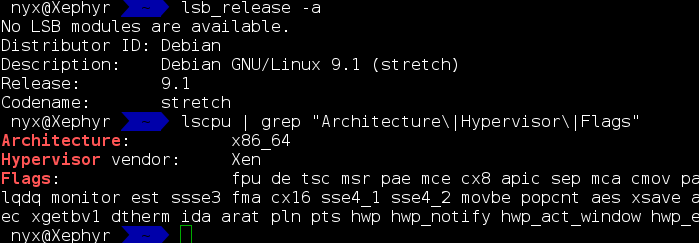
\includegraphics[width=0.75\textwidth]{Figures/sistema-base.png}
    \end{center}
  	\caption{Información del Sistema Base.}
    \label{sistema-base}
\end{figure}

Como se presenta en la figura \ref{sistema-base}, el sistema base para el desarrollo de este trabajo de titulacion utiliza Xen instalado con Debian Stretch (9.1)\footnote{Como el sistema de Dom0} instalado en un LVM con el nombre del grupo de volumenes ''Xephyr-VG''. Originalmente se tenia planificado trabajar con Debian Jessie (8.x) debido que eso fue la version estable al momento de instalacion pero despues se opto por una actualizacion a la version beta de Debian en aquello momento (Debian Stretch). En resumen los pasos realizados fueron:
\lstset{language=Bash}
\begin{enumerate}
	\item Instalacion Limpia de Debian 8 con un LVM.
    	\begin{description}
    		\item[Volumen Fisico:] /dev/sda8 310g 
            \item[Grupo de Volumenes:] Xephyr-VG 310g
            \item[Volumenes Logicos:] Originalmente 4 (se agrega 2 por cada nueva maquina virtual -- uno para su disco y otro para su area de intercambio).
            \begin{description}
            	\item[Xephyr-Dom0] Xephyr-VG 30g
                \item[Xephyr-IMG-Repo] Xephyr-VG 20g
                \item[Xephyr-ISO-Repo] Xephyr-VG 20g
                \item[Xephyr-Swap] Xephyr-VG 4g
            \end{description}
    	\end{description}
    \item Actualizar Instalacion de Debian 8.
    	\begin{lstlisting}
    apt update
    apt upgrade
    apt dist-upgrade
    reboot
        \end{lstlisting}
    \item Actualizar Debian 8 a Debian 9.
        \begin{lstlisting}
    sed -i 's/jessie/stretch/g' /etc/apt/sources.list
    apt update
    apt upgrade
    reboot
        \end{lstlisting}
    \item Instalacion de Herramientas de Trabajo
        \begin{lstlisting}
    apt install tmux vim zsh
        \end{lstlisting}
    \item Instalacion y Configuracion de Hipervisor Xen
		\begin{lstlisting}
    apt install xen-hypervisor
    dpkg-divert --divert /etc/grub.d/08_linux_xen \
    	--rename /etc/grub.d/20_linux_xen
    update-grub
    cat > /etc/network/interfaces.d/xenbr << EOF

    auto xenbr0
    iface xenbr0 inet static
       address 10.10.10.1
       netmask 255.255.255.0
       bridge_ports wlan0

    #other possibly useful options in a\
    	virtualized environment
      #bridge_stp off       # disable \
      		Spanning Tree Protocol
      #bridge_waitport 0    # no delay \
      		before a port becomes available
      #bridge_fd 0          # no forwarding\
      		delay

    ## configure a (separate) bridge for\
    	the DomUs without giving Dom0 an\
        IP on it
    #auto xenbr1
    #iface xenbr1 inet manual
    #   bridge_ports eth1

    EOF

    reboot
		\end{lstlisting}
	\item Instalacion de Herramientas de Xen
		\begin{lstlisting}
	apt install xen-tools xen-utils
		\end{lstlisting}
\end{enumerate}

Estos pasos de instalacion se basaron en la guia de instalacion de Xen publicado en el wiki del proyecto de Debian \citep{Debian-Wiki-Xen}.

\subsection{Ambiente Virtual de LMS (Moodle)}

Para el ambiente de Moodle (LMS contra el cual se ha llevado el desarrollo), se crea una maquina virtual de Debian Stretch (9) con 1 GiB de RAM, 1 CPU virtual, 6 GiB de disco, 512 MiB de intercambio y una direccion IP fija de 10.10.10.10. Los resultados del mismo commando se puede ver en la figura \ref{vm-moodle}.
\begin{lstlisting}
	xen-create-image --hostname=debian-moodle\
    		--ip=10.10.10.10 --netmask=255.255.255.0\
        	--gateway=10.10.10.1 --memory=1024mb\
        	--vcpus=1 --lvm=Xephyr-VG --pygrub\
        	--dist=stretch --force --size=6144mb\
        	--swap=512mb
\end{lstlisting}

\begin{figure}
	\begin{center}
    	%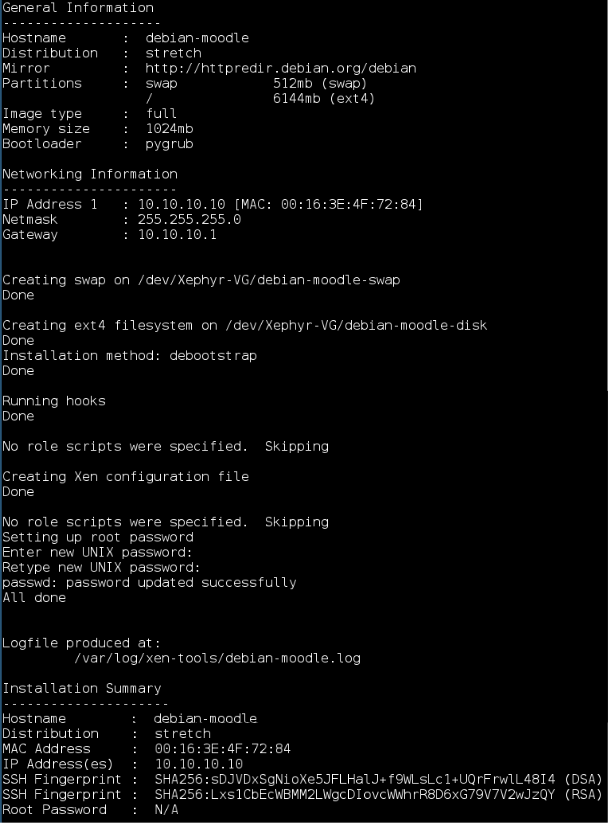
\includegraphics[width=0.75\textwidth]{Figures/crear-moodle.png}
    \end{center}
  	\caption{Crear maquina virtual para Moodle.}
    \label{vm-moodle}
\end{figure}

Se renombró el archivo de configuracion de la maquina virtual generado en el paso anterior para temas de consistencia.

\begin{lstlisting}
	mv /etc/xen/debian-moodle.cfg\
    		/etc/xen/domU-debian-moodle.cfg
\end{lstlisting}

\section{GitEDU}

\subsection{Autenticacion por LTI}

\subsection{Editor de Codigo en Linea}

\subsection{Persistencia de Codigo}

\subsection{Sincronizacion de Notas por LTI}

\subsection{API Externa}

\section{EduNube}

\subsection{Ejeccucion de Codigo en Linea}

\subsection{Calificacion Automatizada con Pruebas Unitarias}

\subsection{API Externa}
